\documentclass[a4paper, 11pt]{article}

\setcounter{tocdepth}{3}
\setcounter{secnumdepth}{3}

\usepackage{comment} % enables the use of multi-line comments (\ifx \fi) 
\usepackage{lipsum} %This package just generates Lorem Ipsum filler text. 
\usepackage{fullpage} % changes the margin
\usepackage[utf8]{inputenc}
\usepackage{gensymb}
\usepackage{graphicx}
\usepackage{booktabs}% http://ctan.org/pkg/booktabs
\usepackage{makecell}
\usepackage{tabularx}
\usepackage[table]{xcolor}
\usepackage{array}
\usepackage{wrapfig}
\usepackage{subcaption}
\usepackage{csquotes}
\usepackage{lscape}
\usepackage{afterpage}
\usepackage{geometry}
\usepackage{listingsutf8}
\usepackage{chngcntr}
\usepackage{multicol}
\usepackage{xcolor}
\usepackage{pifont}


\counterwithin{figure}{section}

\AtBeginDocument{\counterwithin{lstlisting}{section}}

\geometry{a4paper, margin=1in}
\renewcommand{\figurename}{Abb.}
\renewcommand{\tablename}{Tabelle}
\newcommand{\code}[1]{\texttt{#1}}

\renewcommand*{\thead}[1]{\bfseries #1}

\renewcommand{\contentsname}{Inhalt}
\renewcommand{\listfigurename}{Abbildungsverzeichnis}

\definecolor{lightgray}{rgb}{.9,.9,.9}
\definecolor{darkgray}{rgb}{.4,.4,.4}
\definecolor{purple}{rgb}{0.65, 0.12, 0.82}
\definecolor{darkgreen}{rgb}{0.05,0.56,0.06}


\lstset{frame=tlrb,
	language=Java,
	captionpos=b,
	aboveskip=3mm,
	belowskip=3mm,
	showstringspaces=false,
	columns=flexible,
	basicstyle={\small\ttfamily},
	numbers=left,
	numberstyle=\tiny\color{gray},
	keywordstyle=\color{blue},
	commentstyle=\color{violet},
	stringstyle=\color{darkgreen},
	breaklines=true,
	breakatwhitespace=true,
	tabsize=3,
	literate=%
	{Ö}{{\"O}}1
	{Ä}{{\"A}}1
	{Ü}{{\"U}}1
	{ß}{{\ss}}1
	{ü}{{\"u}}1
	{ä}{{\"a}}1
	{ö}{{\"o}}1
}


\begin{document}

\newgeometry{top=0in, bottom=0in}
\title{Zusammenfassung MOBPRO FS2018}
\author{Alex Neher}
\maketitle

\tableofcontents

\newpage
\graphicspath{{./Pictures/}}

\restoregeometry

\section{Grundlagen}
\subsection{Komponenten}
Ein Android-App besteht aus \textit{Komponenten}. Es gibt vier verschiedene Arten von Komponenten:

\begin{description}
	\item[Activity: ] Eine View. Eine Komponente, die etwas macht und ein UI hat. (Mail-App)
	\item[Service: ] Eine Activity ohne UI. Eine Komponente, die etwas im Hintergrund ausführt. (Musikplayer im Hintergrund)
	\item[Broadcast Receiver: ] Event-Listener, der auf Broadcasts und Intents hört und
	 antwortet
	 \item[Content Provider: ] Ermöglicht den Datenaustausch zwischen Applikationen (Mail App darf Bilder von der Galerie auswählen)
\end{description}

\subsection{Android Manifest}
Alle Komponenten müssen im \textbf{Android Manifest} deklariert werden. Das Manifest enthält alle Komponenten der App, welche Intents gesendet und empfangen werden können, welche Permissions die App benötigt und so weiter

\begin{lstlisting}[language=xml, captionpos=b, caption={Einfaches Android-Manifest}]
<?xml version="1.0" encoding="utf-8"?>
<manifest xmlns:android="http://schemas.android.com/apk/res/android"
package="ch.hslu.mobpro.firstapp" >

	<application
		android:allowBackup="false"
		android:icon="@drawable/ic_launcher"
		android:label="@string/app_name"
		android:supportsRtl="true"
		android:theme="@style/AppTheme" >
		<activity android:name="ch.hslu.mobpro.firstapp.MainActivity"
			android:label="FirstApp" >
			<intent-filter>
				<action android:name="android.intent.action.MAIN" />
				<category android:name="android.intent.category.LAUNCHER" />
			</intent-filter>
		</activity>
		<activity android:name="ch.hslu.mobpro.firstapp.LifecycleLogActivity" />
		<activity android:name="ch.hslu.mobpro.firstapp.QuestionActivity" />
	</application>
</manifest>
\end{lstlisting}

\subsection{Intents}
Der Wechsel zwischen Komponenten wird mittels \textbf{Intents} realisiert. Intents sind eine \textit{offene Kommunikation}. Das heisst, der Sender weiss nicht, ob der Empfänger der Kommunikation überhaupt existiert. 

Es wird unterschieden zwischen \textit{impliziten} und \textit{expliziten} Intents. Explizite Intents rufen gezielt eine Klasse auf, während implizite Intents einfach sagen, was getan werden muss (z.B. "ruf mir einen Browser auf", aber es wird nicht spezifiziert, welchen Browser genau). \\

\begin{lstlisting}[captionpos=b, caption={Beispiel eines expliziten Intents}]
Intent myIntent = new Intent(this, Receiver.class);
intent.putExtra("msg", "Hello World");
startActivity(myIntent);
\end{lstlisting}

\begin{lstlisting}[captionpos=b, caption={Beispiel eines impliziten Intents}]
Intent browserCall = new Intent();
broserCall.setAction(Intent.ACTION_VIEW);
browserCall.setData(Uri.parse("http://www.hslu.ch"));
startActivity(browserCall);
\end{lstlisting}

\begin{lstlisting}[captionpos=b, caption={Empfangen und Auswerten eines Intents}]
Intent intent = getIntent();
String msg = intent.getExtras().getString("msg");
displayMessage(msg);
\end{lstlisting}

Implizite Intents benötigen einen \textit{Filter}, in dem potentielle Empfänger deklariert werden. Das System löst implizite Intents anschliessend mit der dafür am besten geeigneten Komponente auf. Welcher Intent am Besten ist, hängt von der Action, der Category und den mitgesendeten Daten ab.
\vspace{10px}

\noindent Über den \textbf{Package-Manager} können z.B. alle möglichen Activities für einen gegebenen Intent abgefragt werden

\begin{lstlisting}[caption={}]
final List<ResolveInfo> resolveList = getPackageManager()
	.queryIntentActivities(getHsluBrowserIntent(), PackageManager.MATCH_DEFAULT_ONLY);
\end{lstlisting}

Man kann z.B. auch eine eigene Action definieren:

\begin{lstlisting}[caption={Erstellung eines eigenen Custom Action}]
public void startCustomIntentOnClick(final View view){
	final Intent customIntent = new Intent(); //<-- Impliziter Intent
	customIntent.setAction(MY_ACTION_SHOW_TEXT);
	customIntent.addCategory(Intent.CATEGORY_DEFAULT);
	customIntent.addCategory(Intent.CATEGORY_LAUNCHER);
	final String myText = "I did stuff with " + MY_ACTION_SHOW_TEXT;
	customIntent.putExtra("text", myText);
	startActivity(customIntent);
}
\end{lstlisting}

\begin{lstlisting}[language=xml, caption={Registrierung des Intent-Filters im Manifest}]
<activity 
	android:name?".Receiver"
	android:label="@string/app_name">
	<intent-filter>
		<action android:name="ch.hslu.mollbpro.actions.SHOW_TEXT"/>
		<category android:name="android.intent.category.LAUNCHER"/>	//Top Level auf Launcher
		<category android:name="android.intennt.category.DEFAULT"/>	//Default Action
		<data android:mimetype="text/plain"/>
	</intent-filter>
\end{lstlisting}

Es kann auch asynchron eine Activity aufgerufen werden, die anschliessend ein Resultat zurückliefert, welches ausgewertet wird:

\begin{lstlisting}[captionpos=b, caption={Beispiel eines asynchronen Methodenaufrufs}]
//mainActivity
Intent intent = new Intent(this, QuestionActivity.class);
intent.putExtra("question", "Und wie läufts so mit der Androidprogrammierung?");
startActivityForResult(intent, MY_REQUEST_CODE);

//QuestionActivity
Intent answerData = new Intent();
answerData.putExtra("answer", answer);
setResult(RESULT_OK, answerData);
finish();

//MainActivity
@Override
protected void onActivityResult(int requestCode, int resultCode, Intent data) {
//resultat verarbeiten
}
\end{lstlisting}

\subsection{Lebenszyklus}
Eine App kann prinzipiell drei states haben:

\begin{description}
	\item[running: ] App läuft im Fokus und Vordergrund
	\item[paused: ] App läuft im Vordergrund aber nicht mehr im Fokus (z.B. wegen Popup)
	\item[stopped: ] App läuft im Hintergrund weiter
\end{description}

Es gibt verschiedene EventListener die bei einer Statusänderung aufgerufen werden können:

\begin{multicols}{3}
	\begin{itemize}
		\item \code{onCreate()}
		\item \code{onDestroy()}
	\columnbreak
		\item \code{onPause()}
		\item \code{onResume()}
	\columnbreak
		\item \code{onStart()}
		\item \code{onStopped()}
	\end{itemize}
\end{multicols}

\section{Benutzerschnittstellen}
\subsection{Layouts}
Layouts sind XML-Dateien, die in der \code{onCreate()}-Methode einer Activity geladen werden. Es gibt grundsätzlich drei verschiedene Layout-Optionen:

\begin{description}
	\item[Linear Layout: ] Komponenten werden in Zeilen oder Spalten linear angeordnet
	\item[Constraint Layout: ] Komponenten werden "aneinadergebunden". Man kann also sagen "Komp. A ist rechts von B und unterhalb von Komp. C"
	\item[ScrollView: ] Möglichkeit für lange Layouts, die länger sind als der Screen. Erlauben nur ein Child (z.B. LinearLayout)
\end{description}
\vspace{10px}

\noindent Das Layout kann entwder als XML definiert werden (einfacher und häufiger) oder als Java-Code. Events können direkt ins XML eingebettet werden, oder sie können über die bereits bekannte Methode des Event-Listeners in java implementiert werden.

\begin{lstlisting}[language=xml, captionpos=b, caption={Button-Definition in XML}]
<Button
	android:id="@+id/main_button_startBrowser"
	android:layout_width="fill_parent"
	android:layout_height="wrap_content"
	android:text="@string/main_buttontext_startBrowser"
	android:onClick="startBrowser" //Einbettung des Event-Listeners
	android:paddingBottom="@dimen/activity_horizontal_margin"
/>
\end{lstlisting}

\begin{lstlisting}[captionpos=b, caption={Button Event-Definition in Java}]
Button button = (Button) findViewById(R.id.main_button_startBrowser)
button.setOnClickListener(new OnClickListener(){
	@Override
	public voidonClick(View v){
		startBrowser();
	}
})
\end{lstlisting}

\subsection{Ressourcen}
Ressourcen wie Strings, Layouts, Bilder, Arrays etc. werden im \code{/res}-Ordner abgelegt. In der XML-Datei kann über den @-Operator darauf zugegriffen werden (\code{@string/value1}). In Java wird über die automatisch generierte \code{R}-Klasse auf Ressourcen zugegriffen (\code{R.layout.activity\textunderscore main}). Es können mehrere Layout- oder String-Dateien erstellt werden z.B. für Portrait und Landscape Mode oder für verschiedene Sprachen.

\subsection{Interaktion mit dem User}
\subsubsection{Options Menu}
Seit Android 3 oder so gibt es rechts oben in einer App normalerweise drei Punkte, über welche das Options-Menu aufgerufen werden kann. 

Das Options Menu-Layout wird wie alle anderen Layouts über ein XML definiert, welches anschliessned im \code{/res}-Ordner abgelegt wird. 

\begin{lstlisting}[language=xml, captionpos=b, caption={Beispiel eines Menu Layouts}]
<menu xmlns:android="http://schemas.android.com/apk/res/android"
	xmln:tools="http://schemas.android.com/tools" tools:context=".MainActivity">
	<item
		android:id="@+id/main_menu_finish"
		android:title="@string/menu_finish">
	</item>
	<item
		android:id="@+id/main_menu_values"
		android:title="@string/menu_ShowValues">
	</item>
</menu>
\end{lstlisting}

Das Menu wird anschliessend mit dem \code{MenuInflater} 'aufgeblasen'

\begin{lstlisting}[captionpos=b, caption={Beispiel des Menu-Inflators}]
@Override
pulic boolean onCreateOptionsMenu (Menu menu){
	suuper.onCreateOptoinsMenu(menu);
	MenuInflater inflater = getManuInflater();
	inflater.inflate(R.menu.menu_main, menu);
	return true;
}
\end{lstlisting}

\subsubsection{Toast}
Ein Toast ist eine kleine Meldung auf dem Bildschirm, die dem User etwas mitteilt. Der User kann aber nicht mit dem Toast interagieren.

\begin{lstlisting}[caption={Toast-Beispiel}]
Toast toast = Toast.makeText(context, "Toast Bsp", Toast.LENGTH_LONG).show();
\end{lstlisting}

\subsubsection{Dialog}
Der Dialog oder Alert ist ein Popup, der dem User eine Information mitteilt und er darauf reagieren muss.

\begin{lstlisting}[caption={Alert-Beispiel}]
AlertDialog.Builder builder = new AlertDialog.Builder(this);
builder.setTitle(R.string.dialog_fire_missiles_title)
	.setMessage(R.string.dialog_fire_missiles)
	.setPositiveButton(R.string.fire, new DialogInterface.OnClickListener() {
		public void onClick(DialogInterface dialog, int id) {
			// FIRE ZE MISSILES!
		}
	})
	.setNegativeButton(R.string.cancel, new DialogInterface.OnClickListener() {
		public void onClick(DialogInterface dialog, int id) {
			// User cancelled the dialog
		}
	});
AlertDialog dialog = builder.create();
dialog.show();
\end{lstlisting}

\subsubsection{Notifications}
Kommen später

\subsection{Adapter}
Adapter nehmen, wie bereits aus APPE/VSK bekannt, Daten, konvertieren sie in ein anderes Format und übergeben sie dem Zielkomponenten.

\begin{lstlisting}[caption={Array-Adapter um String Array in Spinner zu füllen}]
String[] myArray = new String[]{"Fanta", "Cola", "Eistee"};
ArrayAdapter<String> adapter = new ArrayAdapter<String>(this. android.R.layout.of.spinner, myArray);
this.setListAdapter(adapter);
\end{lstlisting}

Alternativ kann man sich den Adapter auch sparen und das direkt im XML des Komponenten (z.B. Spinner) machen:

\begin{lstlisting}[caption={Spinner-Layout mit direkten Füllen}]
<Spinner
	android:id="@+id/main_spinner"
	android:layout_width="match_parent"
	android:layout_height="wrap_content"
	android:entries="@array/itCourses" /> //Füllt das Array in den Spinner
</Spinner>

//in array.xml
<resources>
	<string-array name="itCourses">	
		<item>MOBPRO</item>
	</string-array>
</resources>
\end{lstlisting}

\subsection{Kontextspeicherung}
Der Zustand der App geht verloren, wenn die App gestoppt oder pausiert wird, oder auch wenn  z.B die Bildschirmorientierung geändert wird. Man kann aber bestimmte Daten kurzzeitig im Memory speichern und sie anschliessend wieder abrufen:

\begin{lstlisting}[caption={Abspeichern und Abrufen von Values im Memory}]
//Speichern
@Override
protected void onSaveInstanceState(Bundle outState){
	outState.putInt(KEY, value);
	super.onSaveInstanceState(outState);
}

//Abrufen
@Override protected void onRestoreInstanceState(Bundle savedInstanceState){
	super.onRestoreInstanceState(savedInstanceState);
	value = savedInstanceState.getInt(KEY);
}
\end{lstlisting}

\section{Persistenz}
Es wird grundsätzlich zwischen drei Arten von Präferenzen unterschieden:

\begin{description}
	\item[Default Shared Preferences: ] \code{getDefaultSharedPreferences(this)}. Für die gesamte App
	\item[Shared Preferences: ] \code{getSharedPreferences(name, mode)}. Beliebig viele Präferenzen pro App mit je einem eigenen Namen
	\item[Private Preferences: ] \code{getPreferences(mode)}. Für die aktuelle Aktivität
\end{description}

\begin{lstlisting}[caption={Holen des ResumeCount und um eins erhöht wieder abspeichern}]
final SharedPreferences preferences = getPreferences(MODE_PRIVATE);
final int newResumeCount = preferences.getInt(COUNTER_KEY, 0)+1;
final SharedPreferences.Editor editor = preferences.edit();
editor.putInt(COUNTER_KEY, newResumeCount);
editor.apply();
\end{lstlisting}

\subsection{Dateisysteme}
Dateien können privat oder öffentlich sin. Private Dateien sind ausschliesslich aus der Applikation heras oder über Content Providers zugreifbar und werden im Applikationsverzeich abgelegt. Öffentliche Daten werden auf der SD-Karte oder dem internen Filesystem abgelegt, wo jeder Zugriff drauf haben kann.

\begin{lstlisting}[caption={File schreiben}]
Writer writer = null;
try{
	writer = new BufferedWriter(new FileWriter(outFile));
	writer.write(text);
	return true;
} catch (final IOException ex){
	//catch Exception
}
\end{lstlisting}

Um aufs PUBLIC Filesystem (SD-Karte) zugreifen zu können, muss zuerst eine Berechtigung dafür erlangt werden. Alle Berechtigungen, die eine App benötigt, werden im Android Manifest festgelegt

\begin{lstlisting}[language=xml, caption={Berechtigung im Android Manifest für das Lesen vond der SD-Karte}]
<ises-permission android:name="android.permission.WRITE_EXTERAL_STORAGE"/>
\end{lstlisting}

\begin{lstlisting}[caption={Checken, ob man die Berechtigung hat und wenn nicht, Berechitung anfragen}]
int grant = checkSelfPermission(Manifest.permission.WRITE_EXTERNAL_STORAGE);
if(grant != PackageManager.PERMISSION_GRANTED) {
	requestPermissions(new String[]{Manifest.permission.WRITE_EXTERNAL_STORAGE},23);
} else {
	writeSDCard();
}
\end{lstlisting}

Die Berechtigungen werden über eine Callback-Methode ausgewertet:

\begin{lstlisting}[caption={Verarbeitung der Permission-Grants}]
public void onRequestPermissionsResult(int requestCode, String[] permissions, int[] grantResults){
	switch (requestCode){
		case 24:
			if(grantResults.length > 0 && grantResults[0] != PackageManager.PERMISSION_GRANTED){
				Toast.makeText(this, "Permission " + permissions[0] + " denied!", Toast.LENGTH_SHORT).show();
			} else {
				readSDCard();
			}
\end{lstlisting}

\subsection{SQLite}
SQLite ist ein open source relationales Datenbank-Management System, welches für Android optimiert ist. Man hat pro App beliebig viele Datenbanken, jedoch nur eine Datei pro Datenbank. Über der DB gibt es noch eine Abstraktionsebene, den sog. \textit{Room}. Der Programmierer greift jedoch nur via \code{dbAdapter()} auf die Datenbank bzw. den Room zu:

\begin{lstlisting}[caption={Anwendung des dbAdapters}]
dbAdapter = new DbAdapter(this);
dbAdapter.open();
Note note = dbAdapter.getNote(17);
\end{lstlisting}  


\section{Content Providers}
Wie bereits im ersten Kapitel erwähnt, ermöglicht der Content Provider den Austausch von Daten über Applikationsgrenzen hinweg. Dies indem er mittels eindeuten URIs auf Items (\code{content://anwendung/gruppe/item}) oder Verzeichnisse (\code{content://anwendung/gruppe})) zugreift. Das Android-OS liefert bereits einige in-house Content Provider wie z.B. Kontakte, Kalender o.ä. 

Der Zugriff auf solche Content Providers läuft immer über den \code{ContentResolver} \\ (\code{Context.getContentResolver()}) und gibt stets einen \textit{Cursor} zurück:

\begin{lstlisting}[caption={Auslesen aller SMS mittels Content Provider}]
public void showSMSList(final View view){
	final Cursor cursor = getContentResolver().query(
		Telephony.Sms.Inbox.CONTENT_URI,
		new String[]{
			Telephony.Sms.Inbox._ID,	//SMS-Id
			Telephony.Sms.Inbox.BODY	//SMS-Text
		},
		null,	//selection
		null,	//selection args
		null	//sort order
	);
}
\end{lstlisting}
\vspace{10px}

\noindent Man kann sich auch einen eigenen Content Provider schreiben, wenn man auf andere Daten zugreifen will, die nicht von den systemeigenen Providern abgedeckt werden. 

\begin{itemize}
	\item Klasse muss von \code{android.content.ContentProvider} abgeleitet sein
	\item Klasse muss bei App-Start initiiert werden (z.b. in der \code{onCreate()-Methode})
	\item CRUD-Methoden (zumindest die, die benötigt werden) müssen implementiert werden
	\item Es muss entschieden werden, ob der Provider exportiert werden soll oder nicht (exportiert = auch andere Anwendungen können auf ihn zugreifen und Daten holen)
\end{itemize}


\section{Kommunikation}
\subsection{HTTP}
Die Kommunikation über HTTP läuft über \code{java.net.HttpURLConnection}, der aber davon abhängt, dass man bereits eine URL (\code{java.net.URL}) hat, auf die er verbinden kann:

\begin{lstlisting}[caption={}]
URL url = new URL("www.hslu.ch");
HttpURLConnection httpConnection = (HttpURLConnecton) url.openConnection();
httpConnection.setInstanceFollowRedirects(true);
httpConnection.connect();
if(httpConnection.getResponseCode() == HttpURLConnection.HTTP_OK){
	InputStream content = httpConnection.getInputStream();
	//content verarbeiten
}
\end{lstlisting}

\paragraph{Exkurs: Stream zu Text verarbeiten}\mbox{}\\
Mithilfe eines \code{BufferedReader} kann der \code{InputStream} der HTTP-Connection zeilenweise ausgelesen werden:

\begin{lstlisting}[caption={}]
private String readText(InputStream in) throws IOException{
	StringBuilder text = new StringBuilder();
	String line;
	BufferedReader reader = new BufferedReader(new InputStreamReader(in));
	while((line = reader.readLine()) != null){
		text.append(line);
		text.append("\n");
	}
	reader.close();
	return text.toString();
}
\end{lstlisting}

\subsection{Sockets}
Im Gegensatz zu HTTP sind Sockets \textbf{zustandsbehaftet}, sie merken sich also den Kontext (z.B. Logins). Die Kommunikation basiert auch auf keinem Protokoll wie HTTP, sondern man sendet einfach Datenströme hin und her. Ebenfalls bleibt die Client-Server Verbindung so lange offen, bis sie einer der beiden abbricht.
\vspace{10px}

\noindent Der Ablauf ist prinzipiell so, dass der Server einen Socket hat, auf welchen alle Clients verbinden (quasi eine 'Eingangshalle'). Sobald sich ein Client verbunden hat, wird ein Client-Socket erstellt und der Client wird auf diesen Socket weitergeleitet. Somit ist der Hauptsocket wieder frei für weitere ankommende Verbindungen. 
\vspace{10px}

\noindent Ein Socket wird mittels einer IP-Adresse und einem Port erstellt:

\begin{lstlisting}[caption={Erstellung eines Sockets und dessen Reader/Writer}]
socket = new socket(IP, Port);
writer = new BufferedWriter(new OutputStreamWriter(socket.getOutputStream()));
reader = new BufferedReader(new InputStramReader(socket.getInputStream));
\end{lstlisting}

\section{Nebenläufigkeit}
Java ist zwar multithreaded, aber per Default läuft eine App trotzdem nur auf einem Thread: dem \textbf{main-Thread}, der auch für das UI verantwortlich ist. Soll heissen, wenn der main-Thread blockiert ist, tut das UI keinen Mucks mehr $\rightarrow$ UI-Freeze.

Wenn man nun etwas machen will, was evtl. ein bisschen länger dauern könne und man den UI-Freeze verhindern will, gibt es grundsätzlich zwei Methoden:

\begin{description}
	\item[AsyncTask: ] Die Operation wird gestartet und im Hintergrund ausgeführt. Der main-Thread wird benachrichtigt, sobald ein Resultat vorliegt. Keine eigenen Threads und somit kein nerviges Thread-Handling
	\item[Eigene Threads: ] Man kreiert eigene Threads, so dass die Applikation multithreaded läuft und der main-Thread so nicht überlastat wird. Manchmal notwendig, da der main-Thread z.B. Network-Connections gar nicht zulässt.
\end{description}

\subsection{AsyncTask}
Der AsyncTask ist in drei Methoden aufgeteilt:

\begin{description}
	\item[\code{doInBackground(Params...)}] Lange andauernder Task im Worker-Thread
	\item[onProgressUpdate(Progress...)] Verarbeitung des Zwischenresultates im main-Thread
	\item[onPostExecute(Result)] Verarbeitung des Endresultats im main-Thread
\end{description}

\begin{figure}[htb]
	\centering
	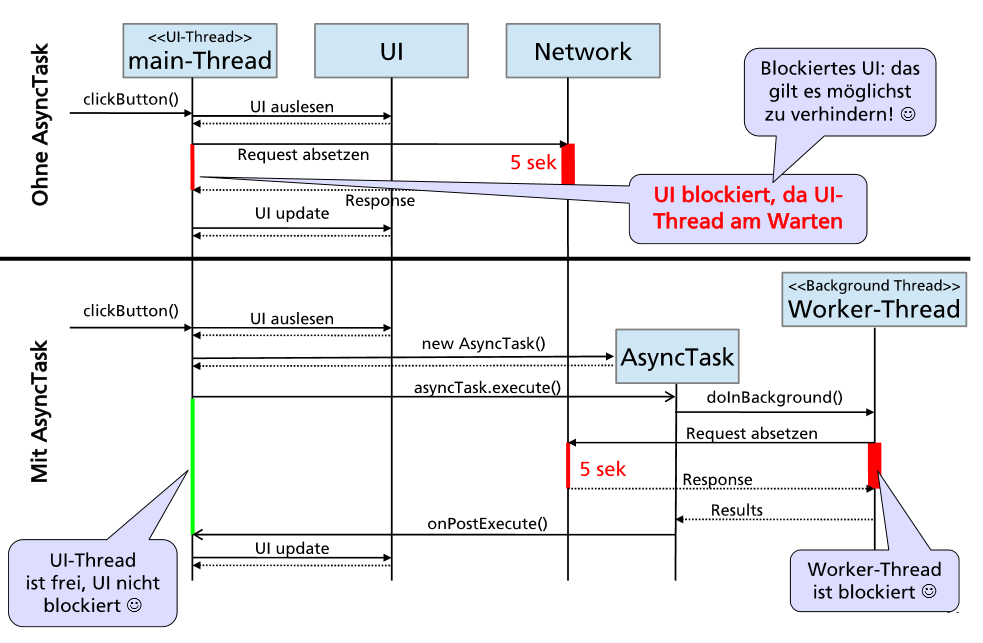
\includegraphics[keepaspectratio=true,height=15\baselineskip]{asynctask}
	\caption{Vergleich mit und ohne AsyncTask}
	\label{fig:asynctask}
\end{figure}

\begin{lstlisting}[caption={}]
														Param, Zwischenresultat, Resultat
public class MultiAsyncTask extends AsyncTask<URL, String, Void>
	@Override
	protected Void doInBackground(URL... urls){		//läuft im Worker-Thread
		try{
			for(URL url : urls){
				InputStram in = openHttpConnection(url);
				String text = readText(in);
				in.close();
				Thread.sleep(WAIT_TIME_MILLIS);
				publishingProgress(text)	//ruft onProgressUpdate auf
			}
		} catch (IOException){
			//do stuff
		}
	}
	
	@Override
	protected void onProgressUpdate(String... values){	//läuft auf main-Thread
		super.onProgressValues(values);
	}
	
	@Override
	protected void onPostExecution(Void result){		//läuft im main-Thread
		AlertDialog.Builder dialogBuilder = new AlertDialog.Builder(mainActivity);
		dialogBiulder
			.//create Dialog with data from URL
	}
	
}
\end{lstlisting}

\subsection{Threads}
Threads sollten (theoretisch) bereits bekannt sein von PRG2 (glaub...), und APPE:
\vspace{10px}

\noindent Die Thread Klasse implementiert das Interface \code{Runnable}, muss also im Konstruktor ein Runnable übergeben werden oder die Methoden \code{run(), start(), sleep(long), isAlive()} selbst implementieren

\begin{lstlisting}[caption={}]
public void startDemoThread(View view){
	final Button button = (Button) view;
	if((demoThread == null) || !(demoThread.isAlive())){
		demoThread = createWaitThread(button);
		demoThread.start();
		button.setText("DemoThread läuft..");
	} else {
		Toast.makeText(this, "DemoThrad läuft schon", Toast.LENGTH_SHORT).show();
	}
}

private Thread createWaitThread(final Button button){
	return new Thrad("hsluDemoThread"){ //<-- Thread-Name
		@Override
		public void run(){
			final Runnable doneRunnable = new Runnable(){
				@Override
				public void run(){
					button.setText("DemoThread starten");
				}
			};
			try{
				Thread.sleep(WAITING_TIME_MILLI) //<-- main-Thread blockiert
				MainActivity.this.runOnUiThread(doneRunnable); // Callback-Benachrichtigung des main-Threads
			}
		}	
	}
}
\end{lstlisting}

\section{Services}
Wie bereits in Kap. 1 erklärt, ist ein Service eigentlich eine Activity, die ohne UI, sprich im Hintergrund durchgeführt wird. Ebenfalls bietet ein Service die Möglichkeit, gewisse Funktionalitäten als API zu exportieren und sie so anderen Apps anzubieten.

Ein Service läuft aber weder auf einem eigenen Thread, noch auf einem eigenen Prozess (ausser man definiert ihn explizit so, z.B. für lange Operationen)
\vspace{10px}

\noindent Services können entweder über \code{startService()} (asynchron) oder \code{bindService()} (synchron) aufgerufen werden:

\begin{multicols}{2}
	\paragraph{\code{startService()}}
	\begin{description}
		\item[\code{onCreate()}] Bei Erzeugung
		\item[\code{onStartCommand()}] Auftragsbehandlung
		\item[\code{onDestroy()}] Bei Beendung (durch System, Service, Applikation oder System)
	\end{description}
\columnbreak
	\paragraph{\code{bindService()}}
	\begin{description}
		\item[\code{onCreate()}] Bei Erzeugung
		\item[\code{onBind()}] Bei Verbindung mit Komponente
		\item[\code{onUnbind()}] Bei Beednung der Verbindung
		\item[\code{onDestroy()}] Bei Beendung (durch System, Service, Applikation oder System)
	\end{description}
\end{multicols}

\begin{lstlisting}[caption={Implementierung und Starten eines Services}]
//Service starten/Auftrag erteilen
Intent musicService = new Intent(this, MyMusicService.class);
musicService.putExtra("audioFileUrl", "http://jurassicpark.org/matingturtles.flac");
startService(musicService);

//Service stoppen
stopService(new Intent(this, MyMusicService.class));

//Service implementieren
public class MyMusicService extends Service{
	@Override
	public int onStartCommand(Intent intent, int flags, int startId){
		startMusicStreamingThreadIfNotRunning();
		String audioFileUrl = intent getStringExtra("audioFileUrl");
		schedulePlay(audioFileUrl);
		return START_STICKY;
	}
}
\end{lstlisting}

\subsection{Service vs. IntentService}
\begin{multicols}{2}
	\paragraph{Service}\mbox{}\\
	Jeder Aufruf von \code{startService()} ruft \code{onStartCommand()} auf. $\rightarrow$ Parallele Abarbeitung
\columnbreak
	\paragraph{IntentService}\mbox{}\\
	Die Aufrufe von \code{startService()} werden gepuffert. $\rightarrow$ Sequenzielle Abarbeitung
\end{multicols}

\subsection{Gebundene Service}
Vorhin wurde die Unterscheidung gemacht zwischen \code{startService()} und \code{bindService()}. Die letztere Methode gehört zu sog. \textit{gebundenen Services}. Diese Services können via \code{ServiceConnection} mit dem Client kommunizieren:

\begin{figure}[htb]
	\centering
	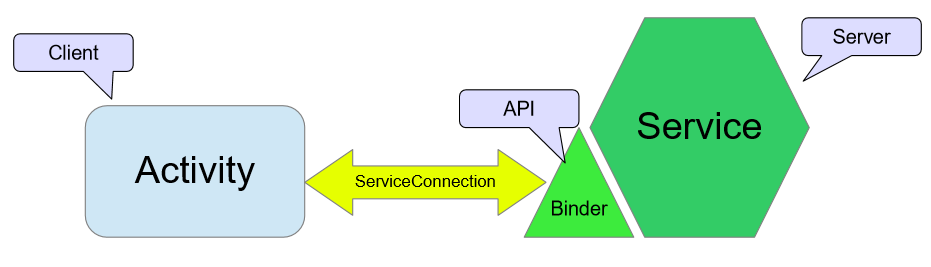
\includegraphics[keepaspectratio=true,height=10\baselineskip]{boundService.PNG}
	\caption{Kommunikation zwischen Activity und gebundenem Service}
	\label{fig:BoundService}
\end{figure}

\begin{figure}[htb]
	\centering
	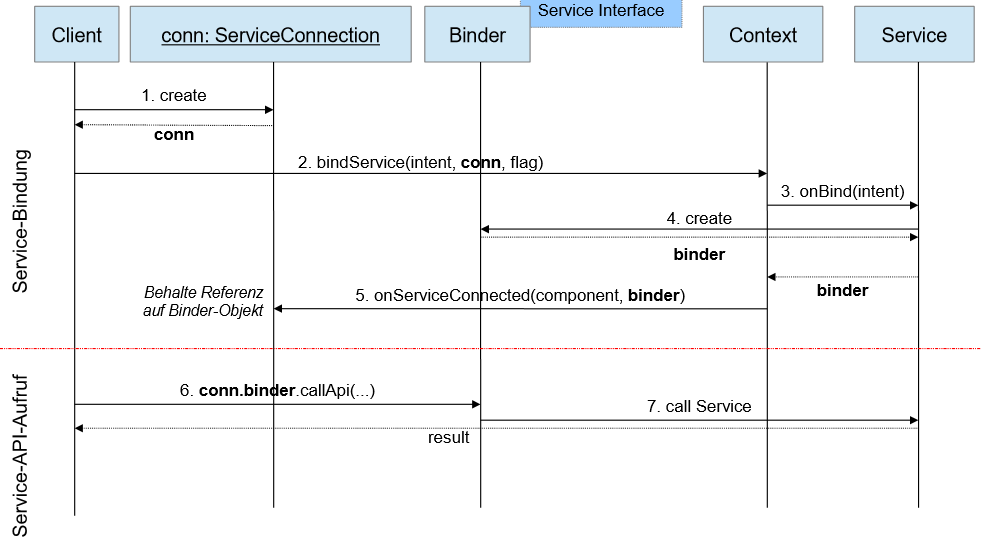
\includegraphics[keepaspectratio=true,height=15\baselineskip]{ablaufBindService.PNG}
	\caption{Wie ein gebundener Service aufgerufen wird}
	\label{fig:ablaufBoundService}
\end{figure}

\section{Broadcast Receiver}
Broadcasts sind essenziell Systemnachrichten wie z.B. \code{BATTERY\textunderscore CHANGED}, \code{BOOT\textunderscore COMPLETED} etc. Prinzipiell können alle Apps Broadcasts via Intents verschicken. Diese verschickten Broadcasts werden von den 'Abonnenten' dieses Broadcasts gesendet.
\vspace{10px}

\noindent Die Bearbeitung eines empfangenen Broadcasts läuft über den \textit{Broadcast Receiver}. Der wird jeweils on-demand erstellt und ist nur so lange aktiv, wie die Bearbeitung des Broadcasts benötigt. Anschliessend wird er wieder gelöscht. 
\vspace{10px}

\noindent Broadcast Receiver müssen auch im Manifest deklariert werden

\begin{lstlisting}[language=xml, caption={BR-Deklaration im Android Manifest}]
<receiver android:name=".BootCompletedReceiver">
	<intent-filer>
		<action android:name="android.intent.action.BOOT_COMPLETED" />
	</intent-filter>
</receiver>
\end{lstlisting}

\begin{lstlisting}[caption={Implementierung eines BR}]
public class BootCompletedReceiver extends BroadcastReceiver {
	@Override
	public void onReceive(Context context, Intent intent){
		//Do stuff
	}
}
\end{lstlisting}

\begin{lstlisting}[caption={Erstellung, Auslösen, Registrierung und Deregistrierung vonv einem BR}]
//Erstellung
BroadcastReceiver timeListener = new BroadCastReceiver(){
	@Override
	public void onReceive(Context context, Intent intent){
		//do Stuff every minute
	}
};

//Registrierung
IntentFilter filter = new IntentFilter("android.intent.action.TIME_TICK");
content.registerReceiver(timeListener, filter);

//BC auslösen
Intent broadcastIntent = new Intent("android.intent.action.TIME_TICK");
sendBroadcast(broadcastIntent);

//Deregistrierung
context.unregisterReceiver(timeListener);
\end{lstlisting}

\section{Widgets}
Widgets zeigen Daten und Funktionalitäten einer App direkt auf dem Home-Bildschirm an. Es gibt unterschiedliche Arten von Widgets:

\begin{figure*}[htb]
	\centering
	\begin{subfigure}[b]{0.5\textwidth}
		\centering
		
\includegraphics[keepaspectratio=true, height=5\baselineskip]{infoWidget.PNG}
		\caption{Informations-Widget}
	\end{subfigure}%
	~ 
	\begin{subfigure}[b]{0.5\textwidth}
		\centering
		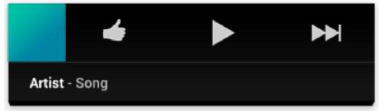
\includegraphics[keepaspectratio=true, height=5\baselineskip]{hybridWidget.PNG}
		\caption{Hybrid-Widget}
	\end{subfigure}
	\vskip\baselineskip
		\begin{subfigure}[b]{0.5\textwidth}
		\centering
		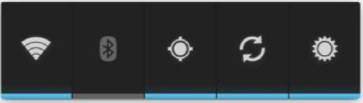
\includegraphics[keepaspectratio=true, height=5\baselineskip]{controlWidget.PNG}
		\caption{Control-Widget}
	\end{subfigure}%
	~ 
	\begin{subfigure}[b]{0.5\textwidth}
		\centering
		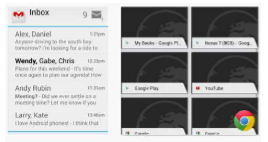
\includegraphics[keepaspectratio=true, height=7.5\baselineskip]{collectionWidget.PNG}
		\caption{Collection-Widget}
	\end{subfigure}
\end{figure*}

Widgets sind spezielle BroadcastReceiver und müssen im Android Manifest deklariert werden. Dazu muss entweder das XML oder die Java-Klasse angegeben werden.

\begin{lstlisting}[language=xml, caption={Widget Deklaration im Manifest}]
<receiver android:name=?".MyAppWidgetProvider"/>
	<intent-filter>
		<action android:name="anddroid.appwidget.action.APPWIDGET_UPDATE"/>
	</intent-filter>
	<meta-data
		android:name="android.appwidget.provider"
		android:resource="@xml/my_app_widget_provider_info />
</receiver>
\end{lstlisting}

\begin{lstlisting}[caption={Widget-Klasse}]
public class MyAppWidgetProvider expends AppWidgetProvider{
	@Override
	public void onUpdate(final Context contex final AppWidgetManager appWidgetManager, fial int[] appWidgetIds){
		for(final int appWidgetId : appWidgetIds){
			final RemoteViews view = new RemoteViews(context.getPackageName(), R.layout.my_app_widget_provider);
			views.setTextViewText(R.id.appwidget_text, "My AppWidget");
			appWidgetManager.updateAppWidget(appWidgetId, views);
		}
	}
}
\end{lstlisting}

\section{Fragments}
\begin{figure}[htb]
	\centering
	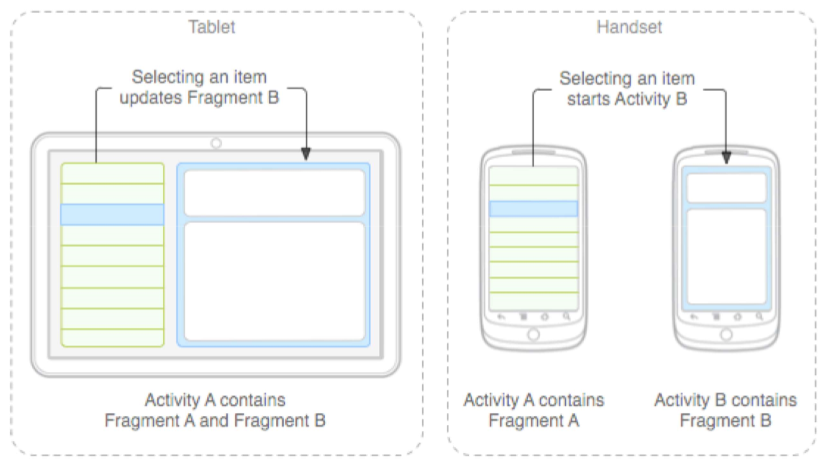
\includegraphics[keepaspectratio=true,height=15\baselineskip]{fragments.PNG}
	\caption{Fragments auf einem Handy und auf einem Tablet}
	\label{fig:fragments}
\end{figure}

Das Ziel von Fragments ist die verbesserte Unterstützung von Tablet-Layouts. Sie sind ein modularer Teil einer Activity, haben einen eigenen Lebenszyklus, einen eigenen Zustand und können zu einer Activity hinzugefügt und wieder entfernt werder mittels Transactions. $\rightarrow$ Fragments sind quasi Sub-Activities, die in verschiedenen Activities wiederverwendet werden können.
\vspace{10px}

\noindent Der Lebenszyklus eines Fragments ist vergleichbar mit dem einer Activity, ausser dass er an eine Activity angehängt wird. Das heisst vor dem \code{onCreate()} muss noch \code{onAttach()} aufgerufen werden.

Gleich wie bei z.B. Options-Menus wird ein Fragment auch mithilfe eines Inflaters (LayoutInflator) 'aufgeblasen'

\vspace{10px}

\noindent Fragments können entweder mit Java-Code oder via XML an eine Activity attached.

\paragraph{Java-Code}\mbox{}\\
\begin{lstlisting}[caption={Attachen eines Fragments im Java-Code}]
public class SetColorActivity extends Activity {
	@Override
	protected void onCreate(Bundle savedINstanceState){
		super.onCreate(savedInstanceState);
		setContentView(R.layout.activity_set_color);
		
		getFragmentManager()
			.beginTransaction()
			.add(R.id.fragmentContainer, FavoriteColorFragment.newInstance())
			.commit();
	}
}
\end{lstlisting}

\paragraph{XML}\mbox{}\\
\begin{lstlisting}[caption={Attachen eines Fragments direkt im XML}]
<TextView
	//Some shit
/>
<Fragment
	android:id="@+id/fragmentFavoriteColor"
	class="ch.hslu.mobpro.intentandwidget.FavoriteColorFragment"
	android:layout_width="match_parent"
	android:layout_height="wrap_content"
	tools:layout="@layout/fragment_favorit_color" />
<Button
	//Some more shit
/>

\end{lstlisting}

\section{App-Design}
Brauche die App-Bar von Google und Googles Material Design und you're good to go

\begin{figure}[htb]
	\centering
	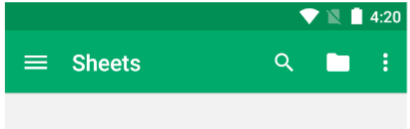
\includegraphics[keepaspectratio=true,height=5\baselineskip]{app_bar.PNG}
	\caption{AppBar}
	\label{fig:appbar}
\end{figure}

\section{Usability und Prototypes}
Mach Prototypen um das App besser durchdacht zu machen.

\section{Support Library}
Die Support Library ermöglicht die Verwendung von neuen Android-Features auch in älteren Android-Versionen, in welchen diese theoretisch nicht (mehr) unterstützt werden.

\section{App-Publizierung}
\begin{multicols}{2}
	\begin{enumerate}
		\item Code Cleanup, Release-Vorbereitung
		\item Release erstellen und signieren
		\item Werbematerial vorbereiten
	\columnbreak
		\item Distributionseinstellungen setzen
			\subitem Altersfreigabe
			\subitem Geo-Verfügbarkeit
			\subitem Kostenpflichtig/In-App Purchases
		\item Release hochladen und publizieren
	\end{enumerate}
\end{multicols}

\begin{description}
	\item[APK: ] Android Application Package, signiertes ZIP mit App drin
	\item[ProGuard: ] Code-Obfuscation und -komprimierung
\end{description}

Apps, die im Google Play Store angeboten werden, müssen mit einem Key signiert sein. Dieser Key muss auch bei der Einspielung von Updates verwendet werden. Wenn der Key verloren geht, hat man keinen Zugriff mehr auf die App und muss sie neu publizieren unter einem anderen Key. Alternativ kann die App auch über andere Websites vertrieben werden, was aber evtl. weniger Kunden bedeutet.



\end{document}
